
To properly evaluate the practical downstream metrics described in section \ref{section:model-evaluation} on model predictions, one must be able to segment nuclei from fluorescence (as well as from predictions) first. Segmentation in this context refers to the creation of a mask. It should consist of $0$s and $1$s,  with a one being assigned to every pixel that is a part of the nucleus, while all the other ones are assigned with a zero. Although this might be a straightforward task for our eyes, it is not that easy to select separate nuclei via postprocessing. There are several edge cases where the nuclei are difficult to segment.

Even though the most extreme corruptions mentioned in section \ref{section:nuclei-preprocessing} were filtered out, some of the images that are corrupted not as severely (meaning they still have all the visible features needed for learning) are still present in the dataset, hence avoiding significant reduction of the amount of data.
\begin{figure}[H]
    \centering
    \setkeys{Gin}{width=\linewidth}
    \centering
        \begin{tabularx}{\textwidth}{YYYY}
            \textbf{Too few cells} &
            \textbf{Overexposure} &
            \textbf{Light gradient} &
            \textbf{Normal lighting} \\
            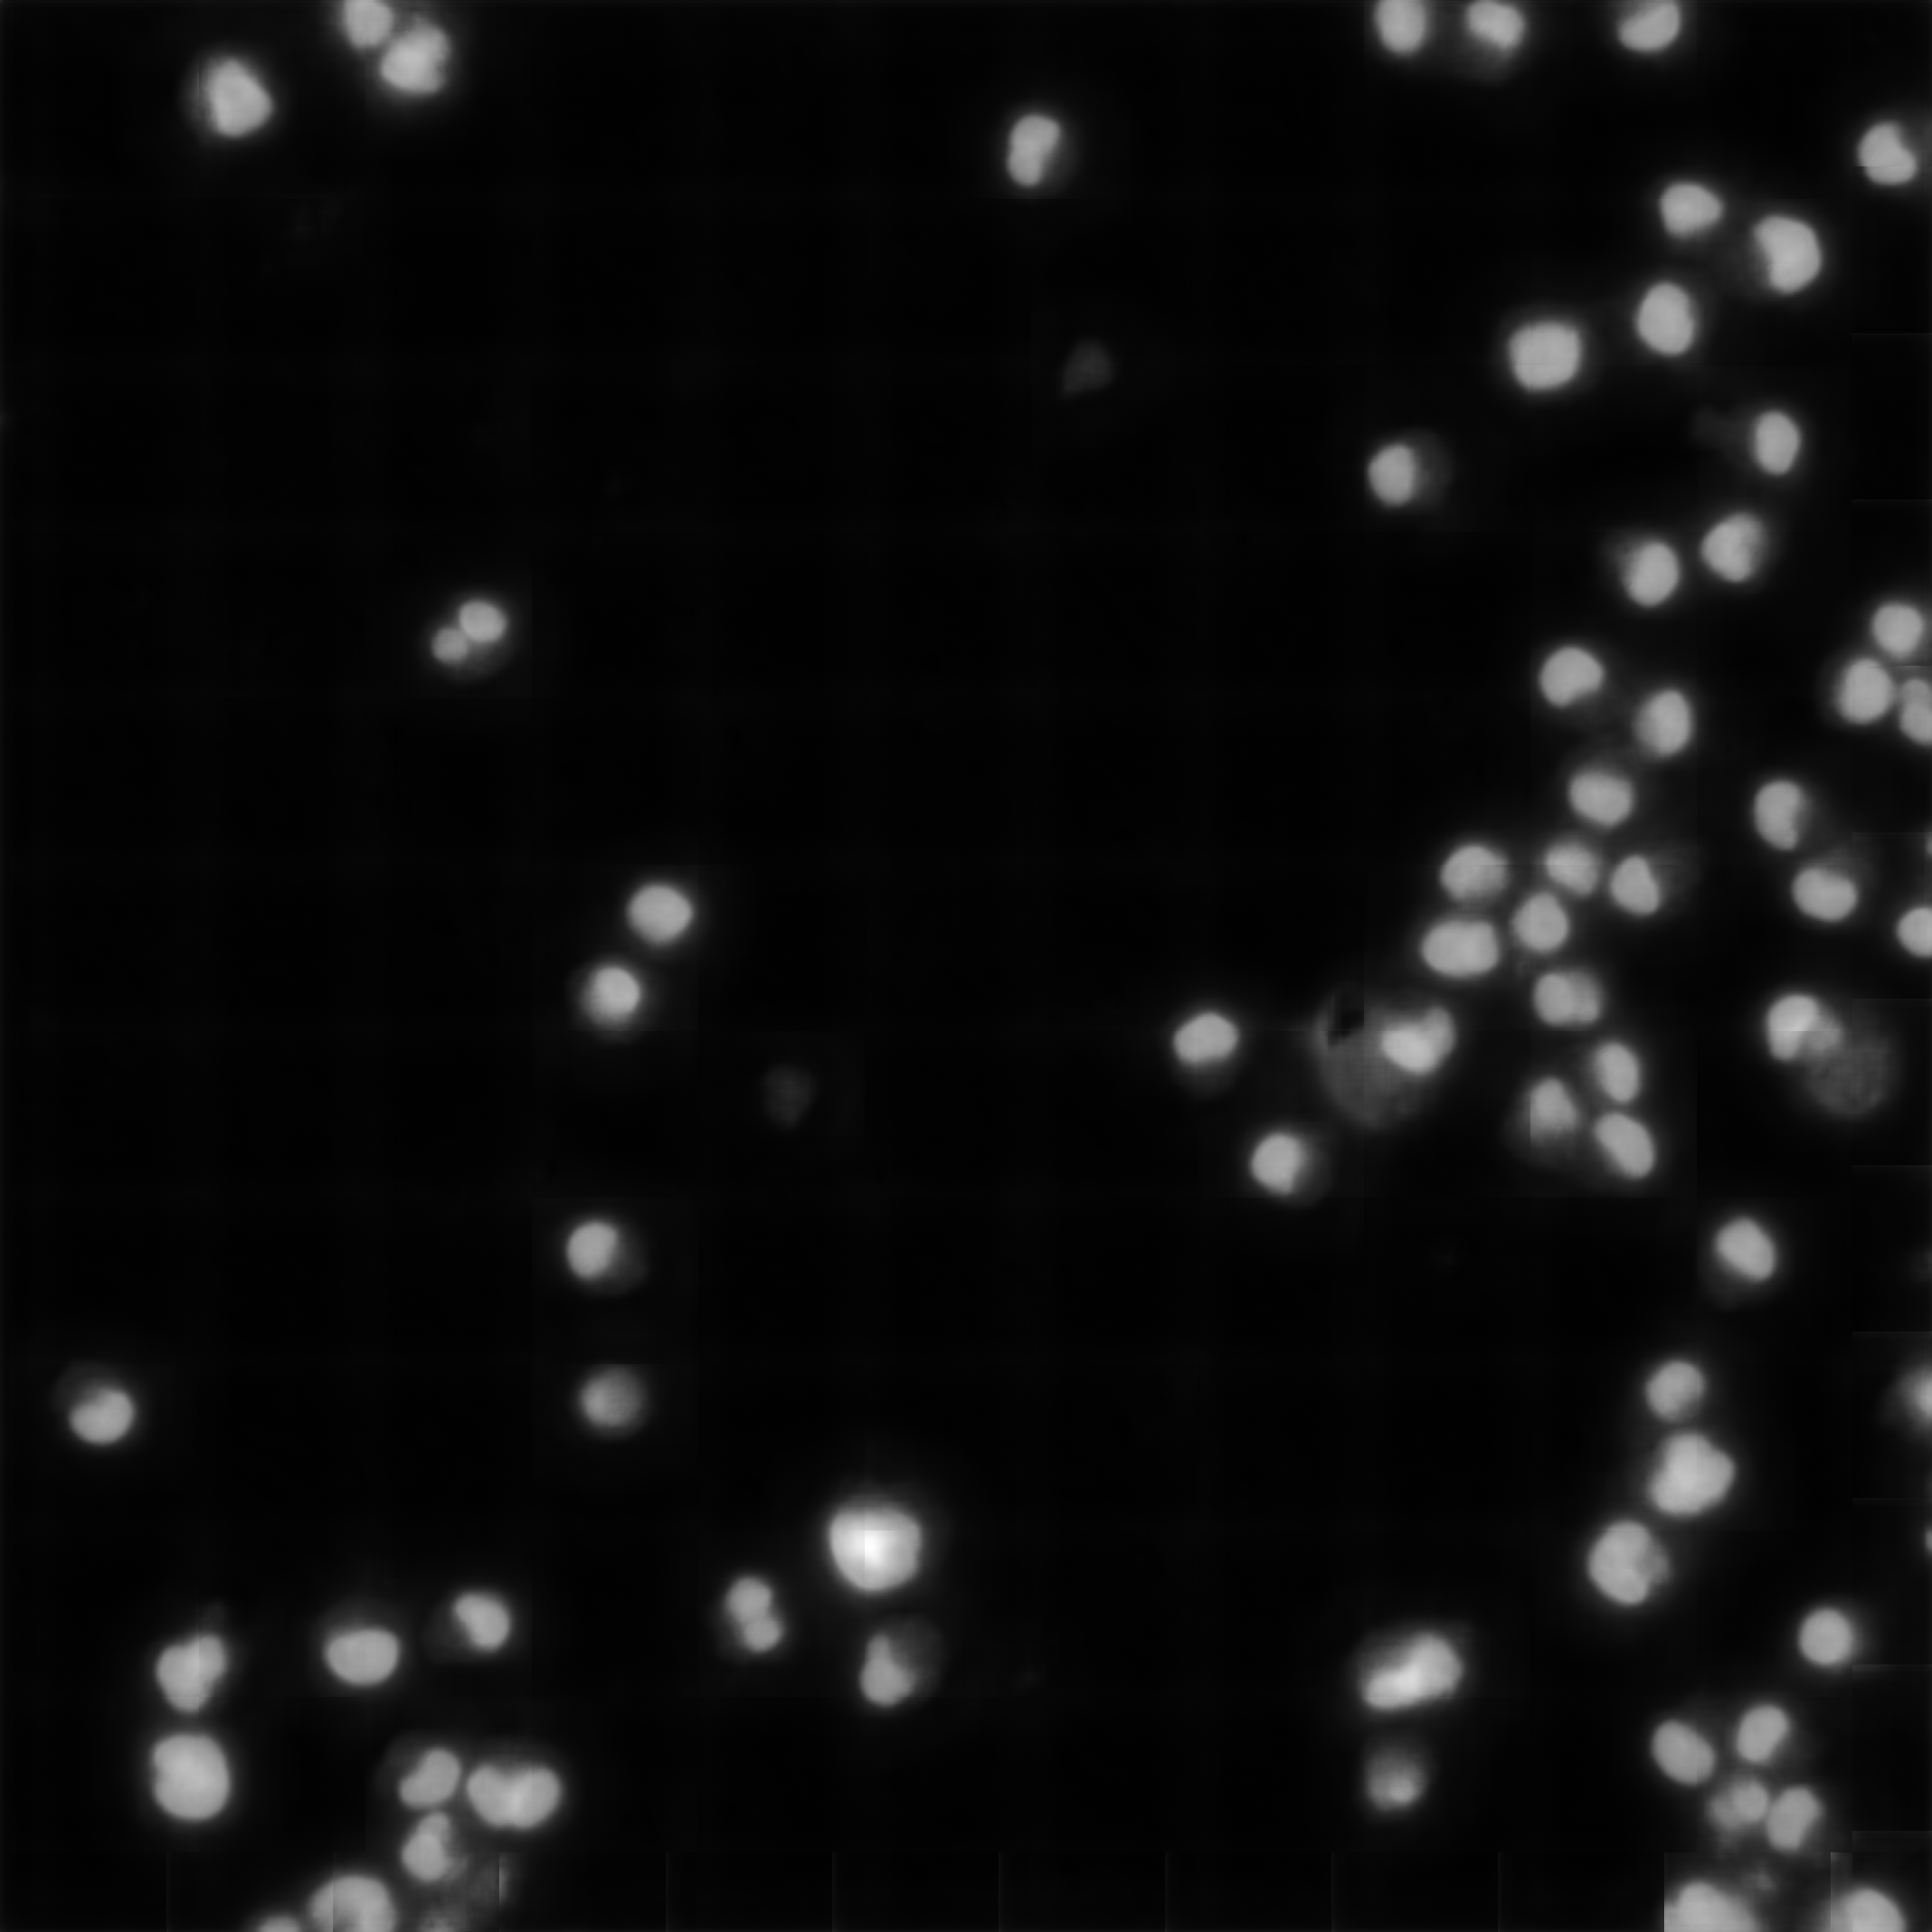
\includegraphics{bilder/lightning-conditions/lightning-1.png} & 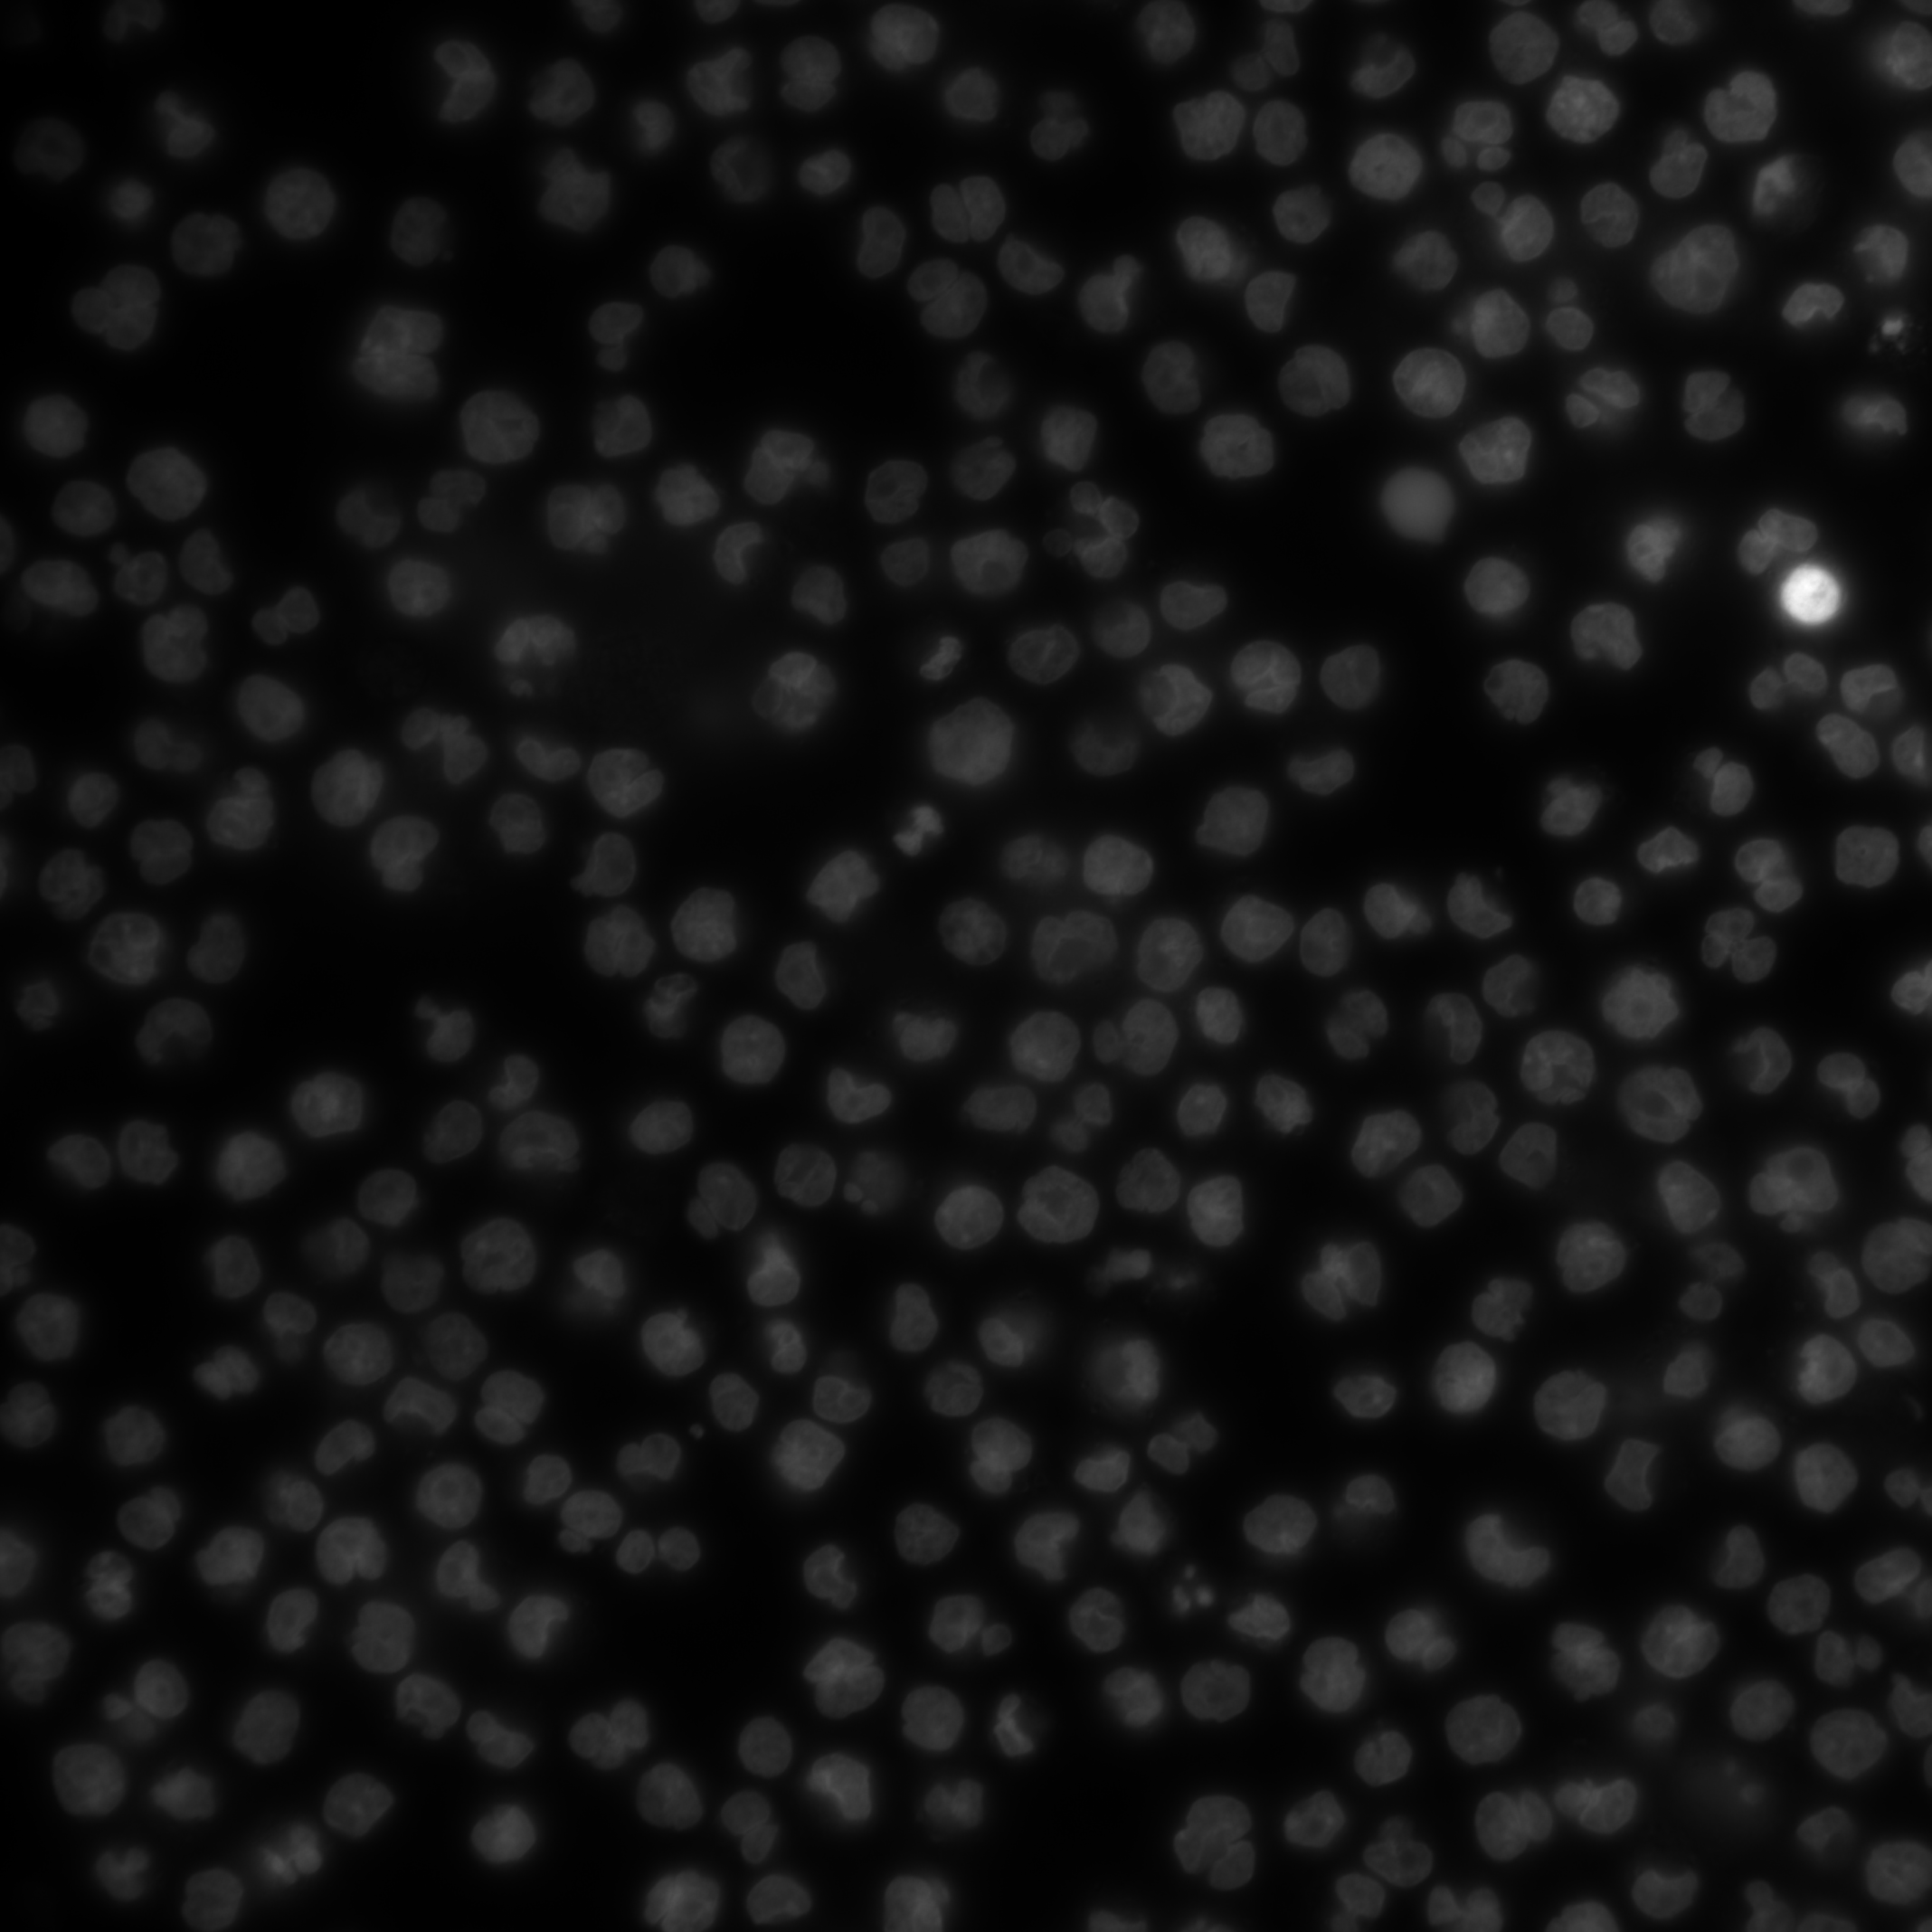
\includegraphics{bilder/lightning-conditions/lightning-2.png} &
            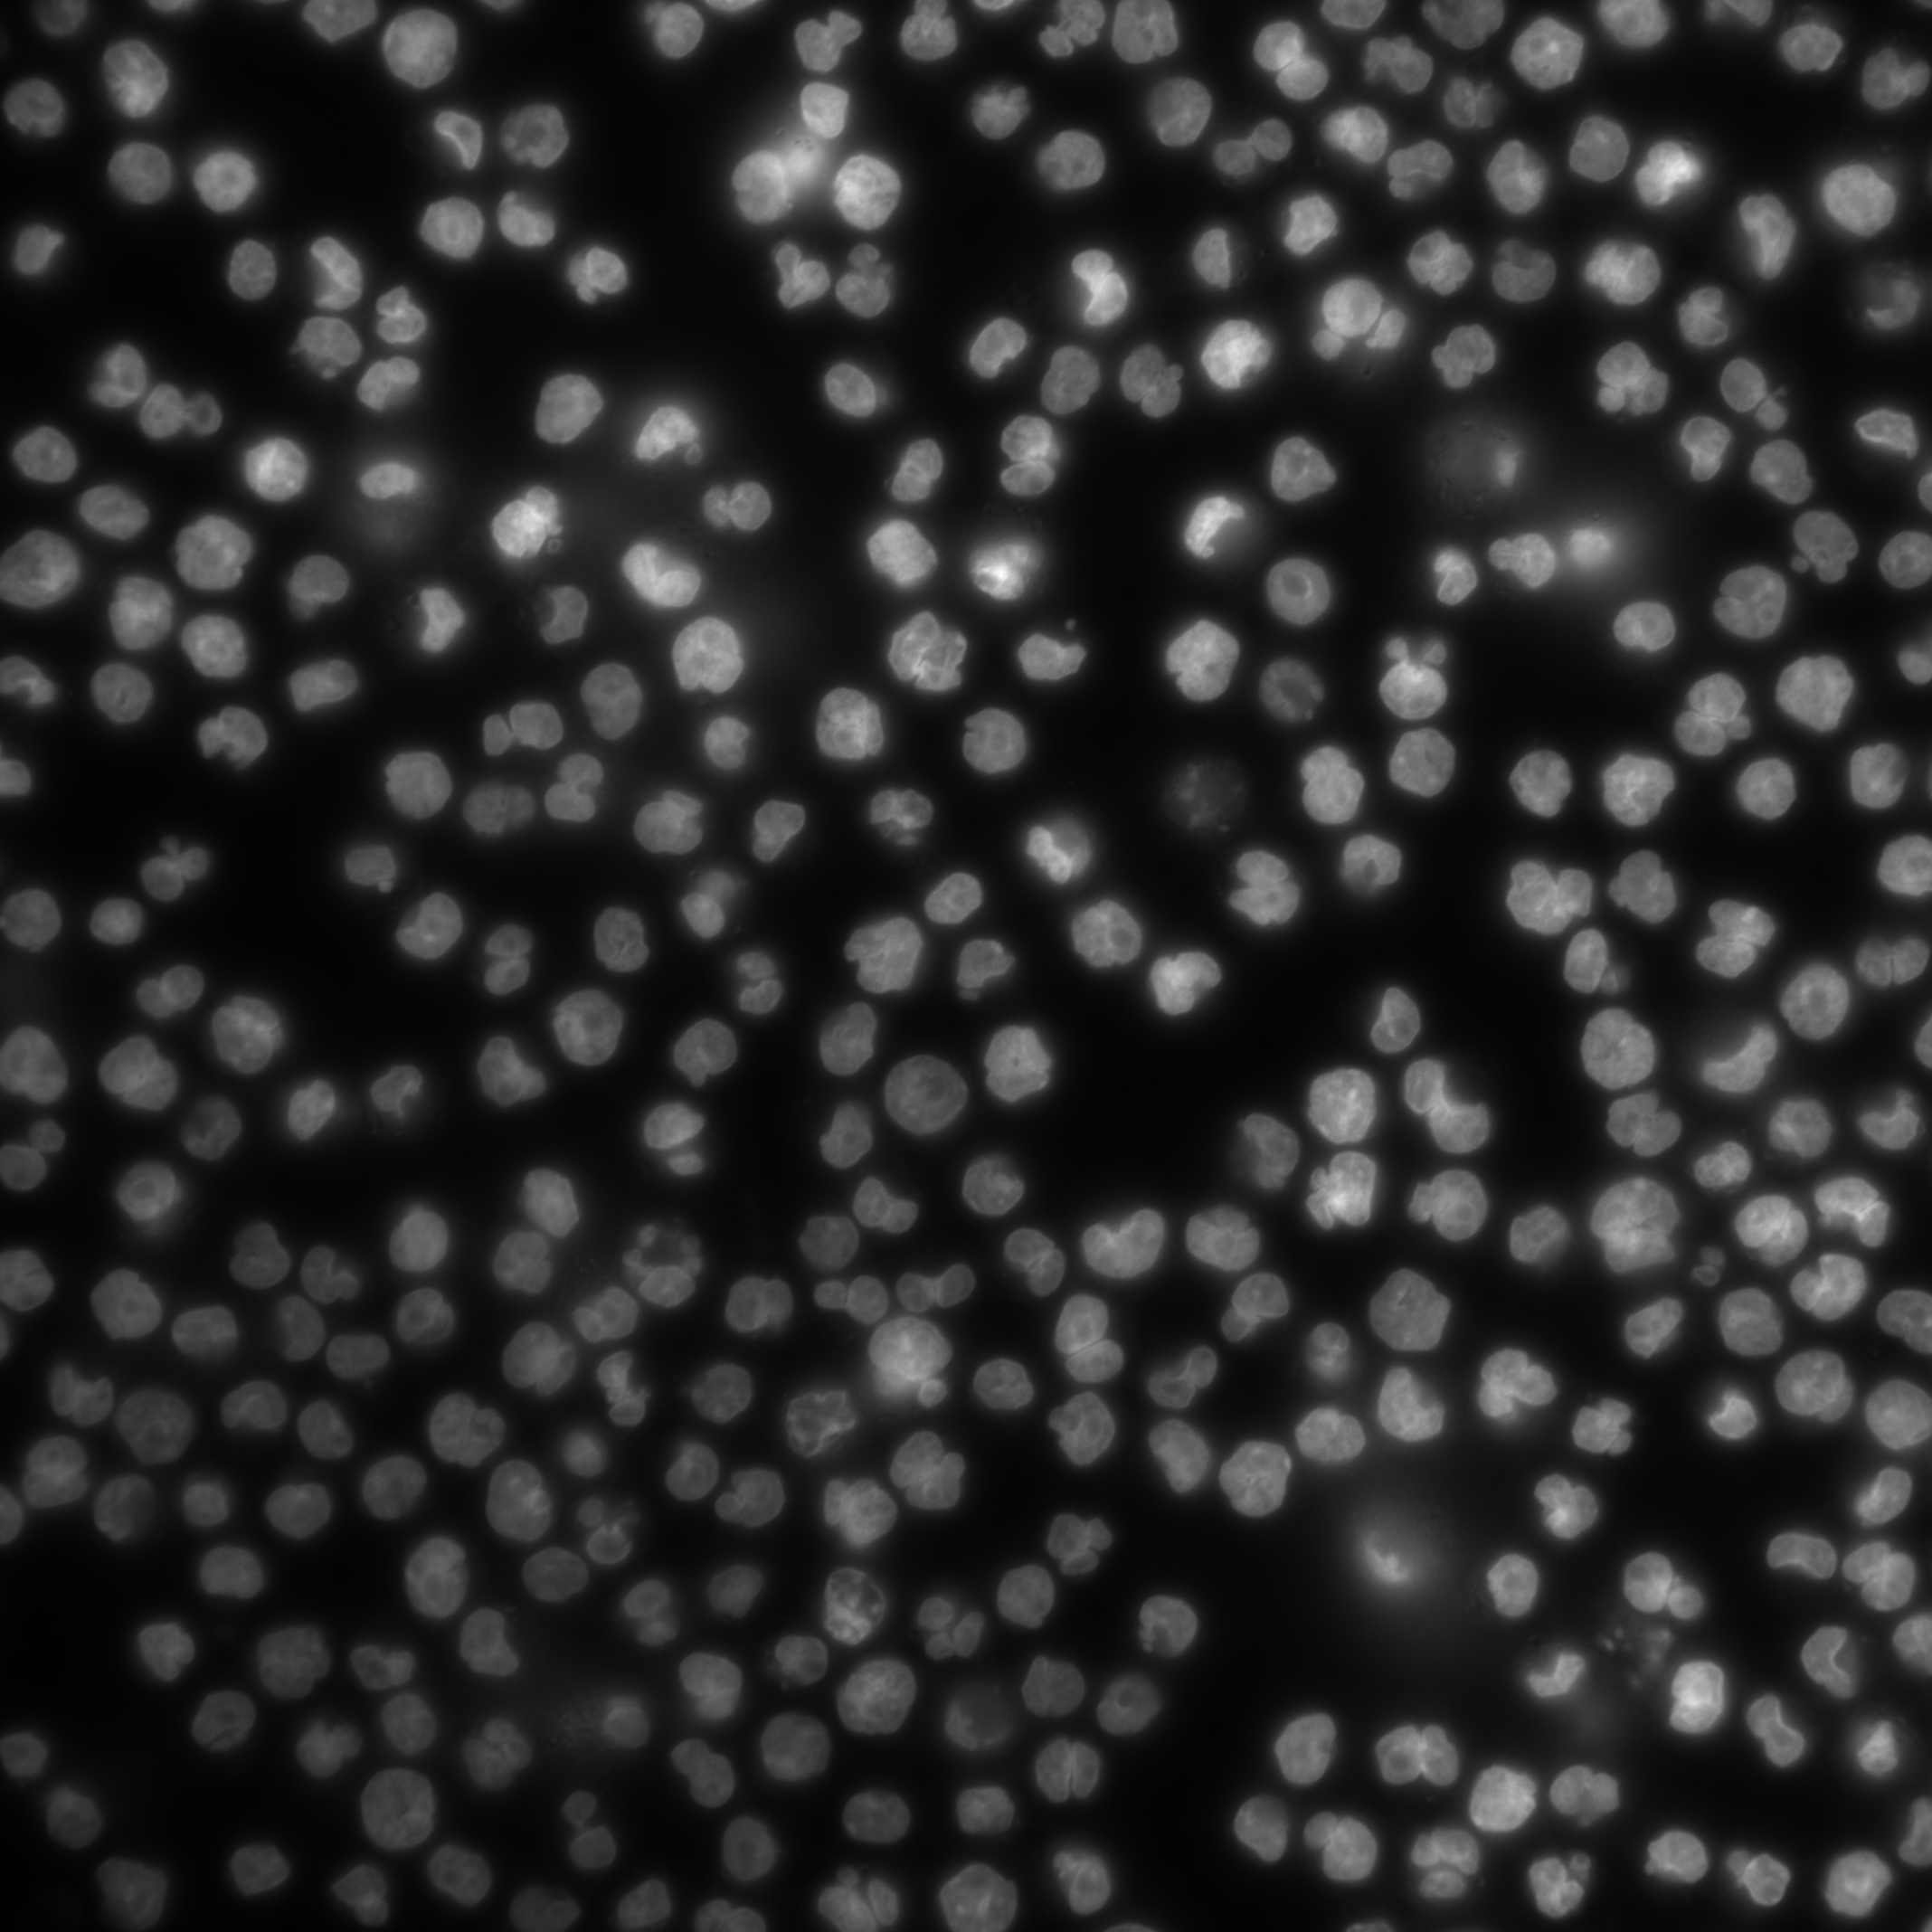
\includegraphics{bilder/lightning-conditions/lightning-3.png} &
            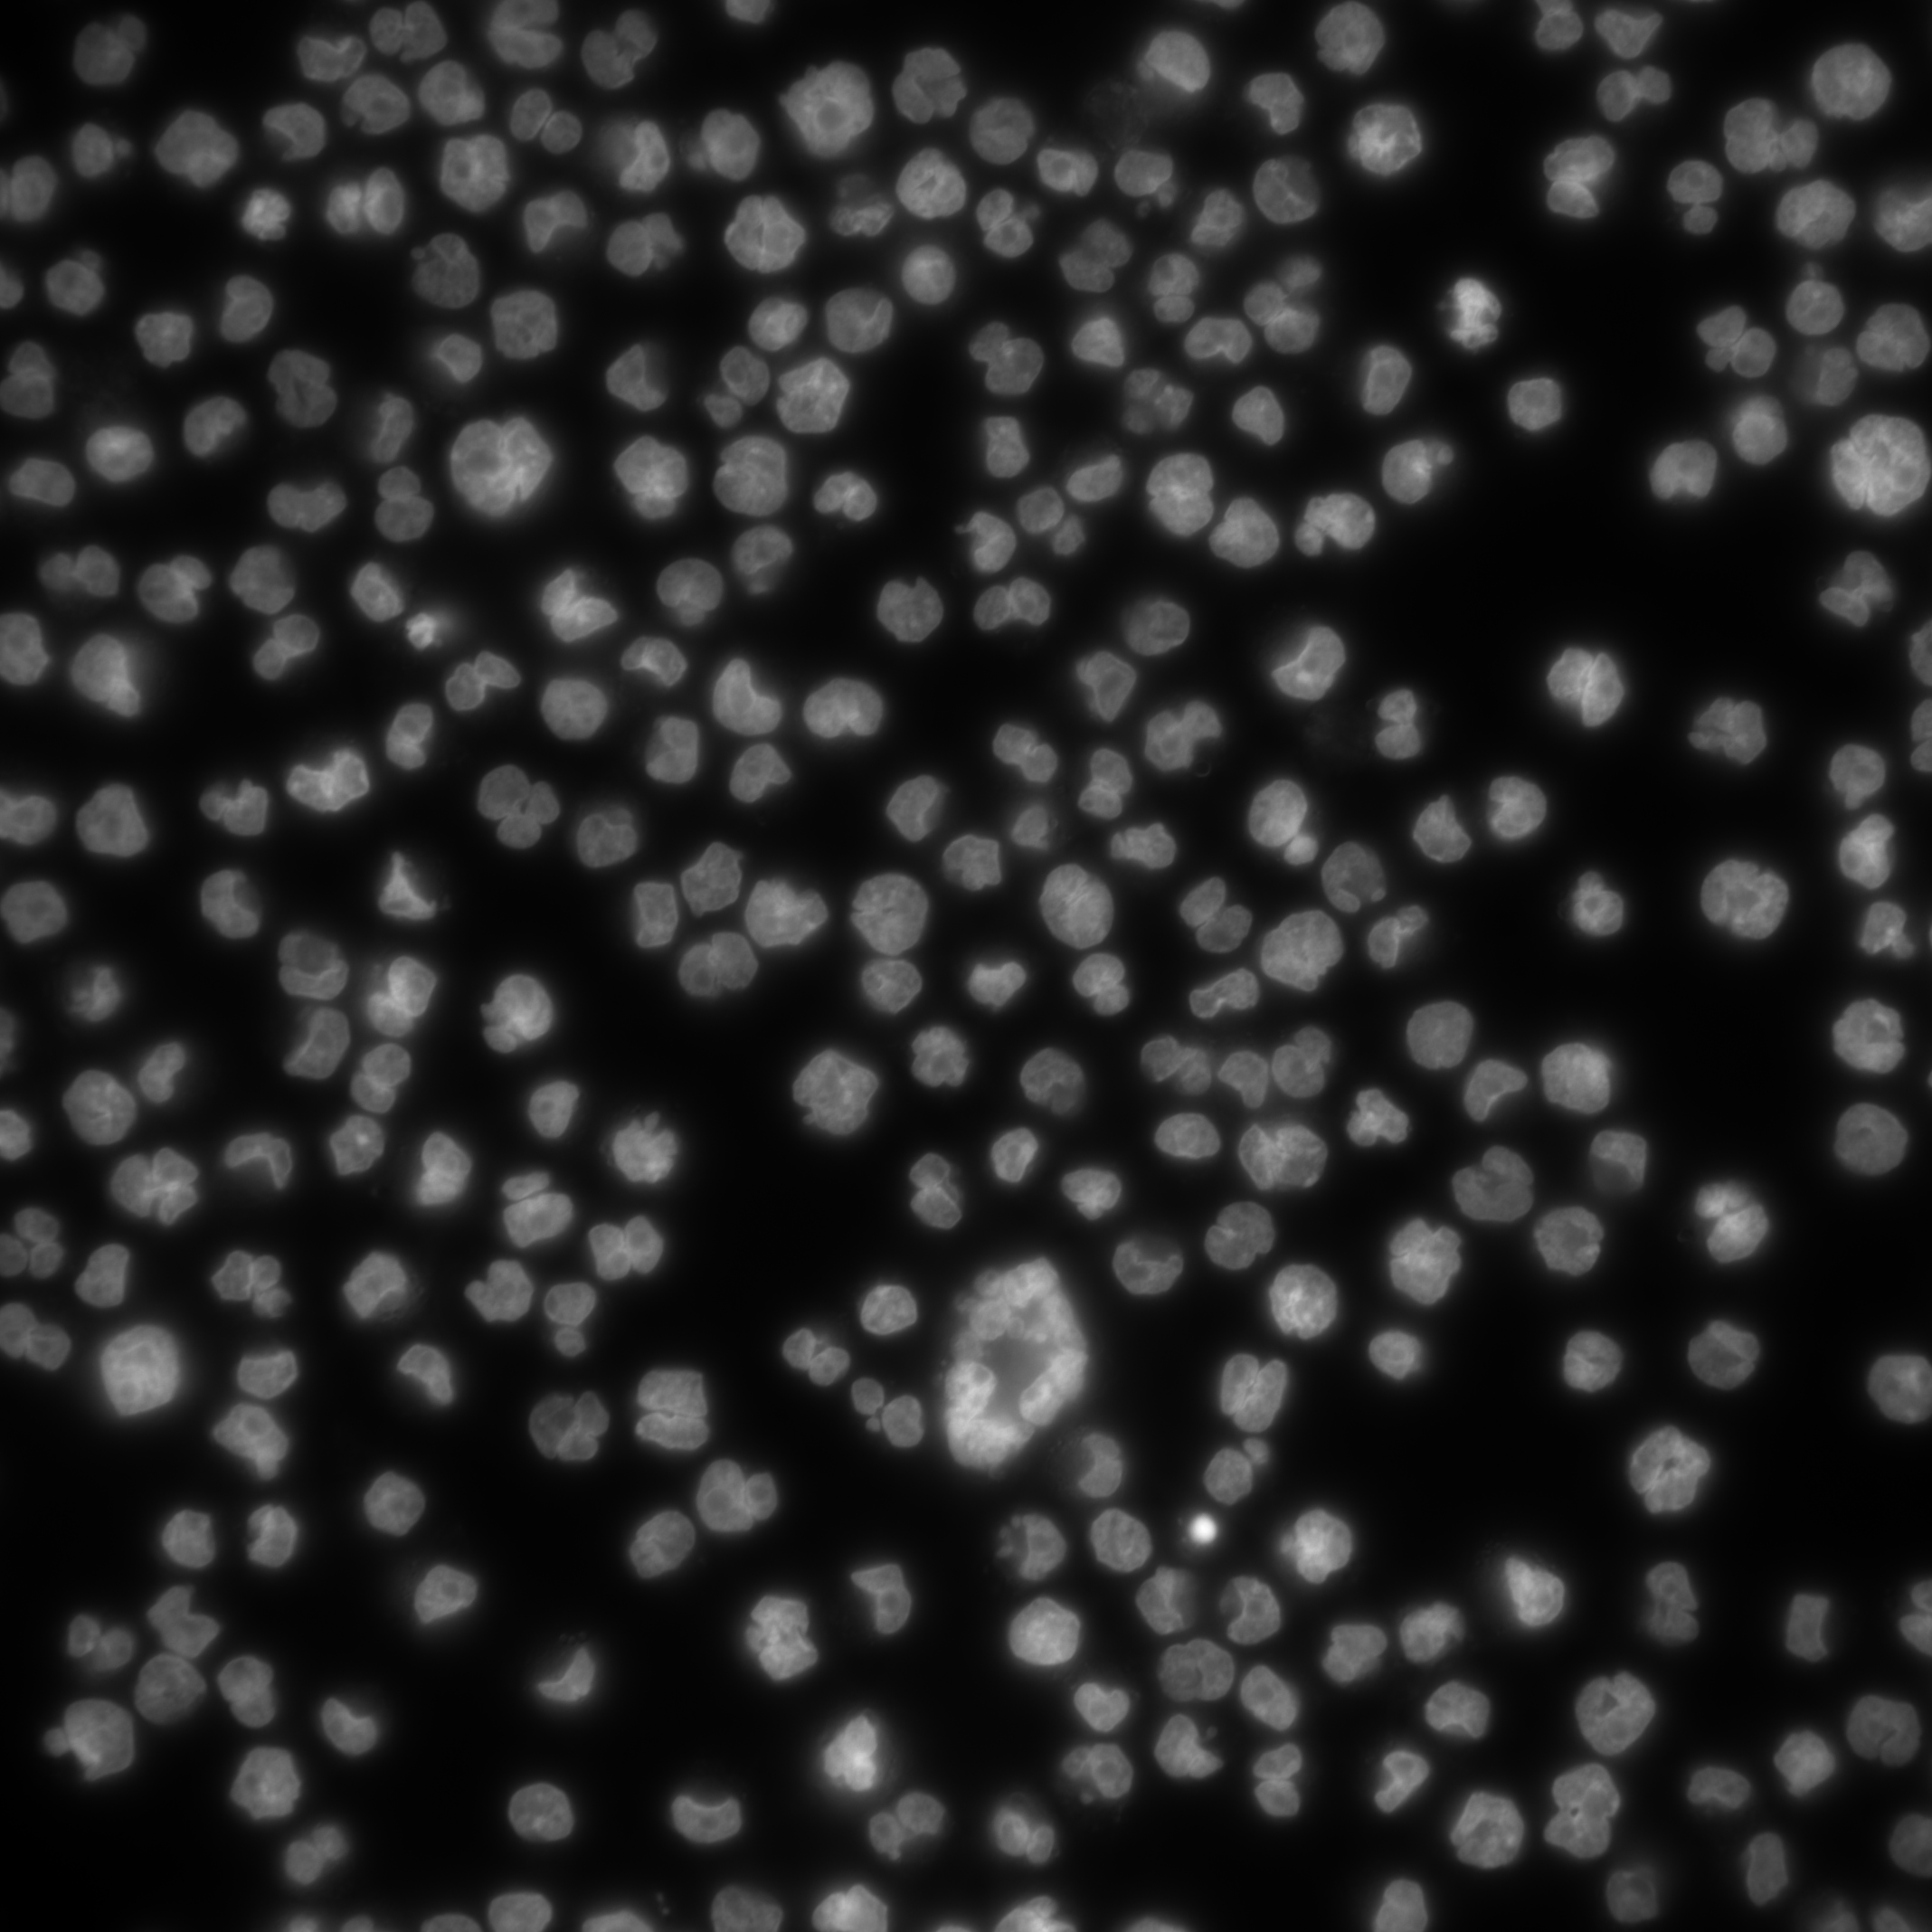
\includegraphics{bilder/lightning-conditions/lightning-4.png}
        \end{tabularx}
    \caption{Different lighting conditions}
    \label{fig:lightning_conditions}
\end{figure}

Examples of cases difficult for segmentation are presented in Figure \ref{fig:lightning_conditions} from left to right: the first image there are too few cells, which leads to the background being much darker than usual; the overexposure of one cell leads to difficulties segmenting the rest of the cells as they are hard to distinguish from the background; lighting gradient from darker (bottom left corner) to brighter (top right corner) region; normal lighting conditions.

Another challenge for segmentation bring nuclei that are very close to each other. This might happen sometimes because some of the cells are currently in the process of division. Also, when some have already fully divided, they might still be located close to one another. The example of such situations is presented in Figure \ref{fig:closely-located-cells}.

\begin{figure}[H]
    \centering
    \subfloat[Original fluorescence]{{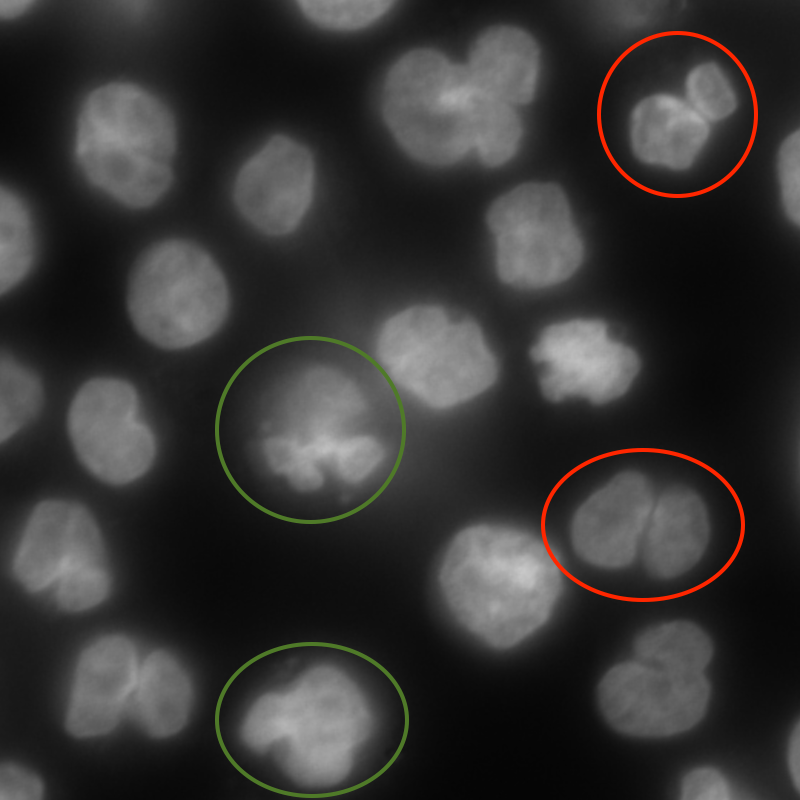
\includegraphics[width=0.2\linewidth]{bilder/close-located-cells/original.png} }}
    \qquad
    \subfloat[Segmentation (violet mask)]{{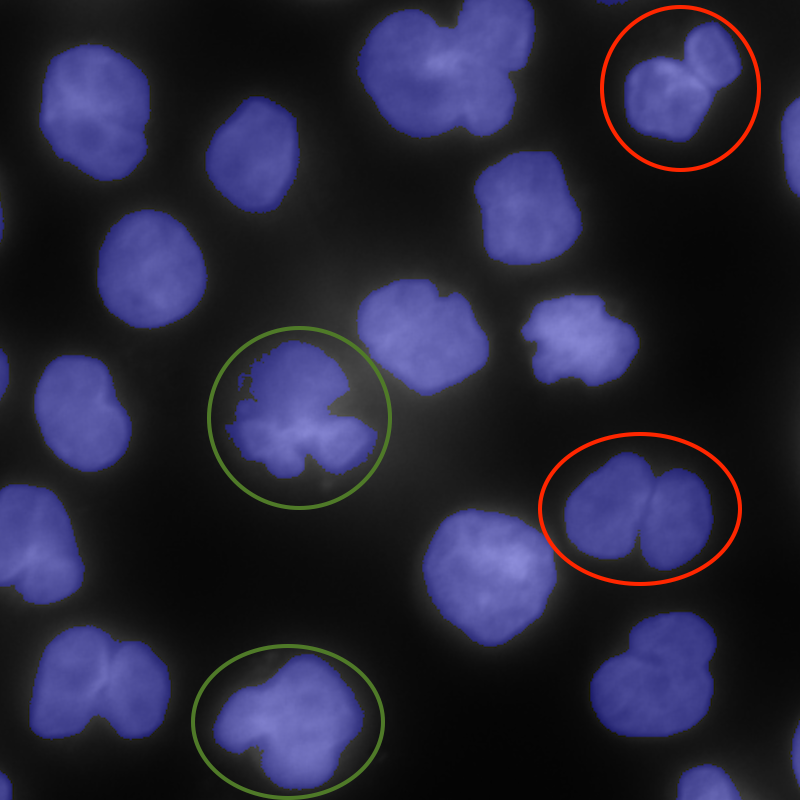
\includegraphics[width=0.2\linewidth]{bilder/close-located-cells/segmented.png} }}
    \caption{Closely located and dividing cells}
    \label{fig:closely-located-cells}
\end{figure}

Here, the cells that are not yet fully divided are highlighted with green circles and the ones that are fully divided, but located too close to one another, are highlighted with red circles. You can see that the segmentation algorithm (see Algorithm \ref{algorithm:nuclei-segmentation}) recognises both such cases as one nucleus. This algorithm is described below and its steps are visualized in Figure \ref{fig:segmentation-nuclei-steps}.
\begin{algorithm}
    \caption{Fluorescence segmentation}
    \begin{algorithmic}
    \item 1. Normalize image.
    \item 2. Apply local thresholding and get a threshold $T$ or a set of local thresholds \{$T_i$\} and create an initial mask: $1$ if $x_i > T$ or $0$ otherwise.
    \item 3. Apply \textit{fill\_holes} transformation to the initial mask in order to get rid of unneeded details within the nuclei.
    \item 4. Run \textit{findContours} from opencv in order to obtain separate regions and filter them based on the following criteria: filter out regions that are too big (measure the biggest possible nuclei manually), regions that are too small (measured manually as well), regions that have a shape that is not similar to convex circular type of nuclei. The last filter is done by checking the ratio of the area of the region to the area of the convex hull of the region.
    \end{algorithmic}
    \label{algorithm:nuclei-segmentation}
\end{algorithm}

\begin{figure}[htb]
    \centering
    \setkeys{Gin}{width=\linewidth}
    \centering
        \begin{tabularx}{\textwidth}{YYYY}
            \textbf{Normalized input} &
            \textbf{Local threshold} &
            \textbf{Filled holes} &
            \textbf{Filtered regions} \\
            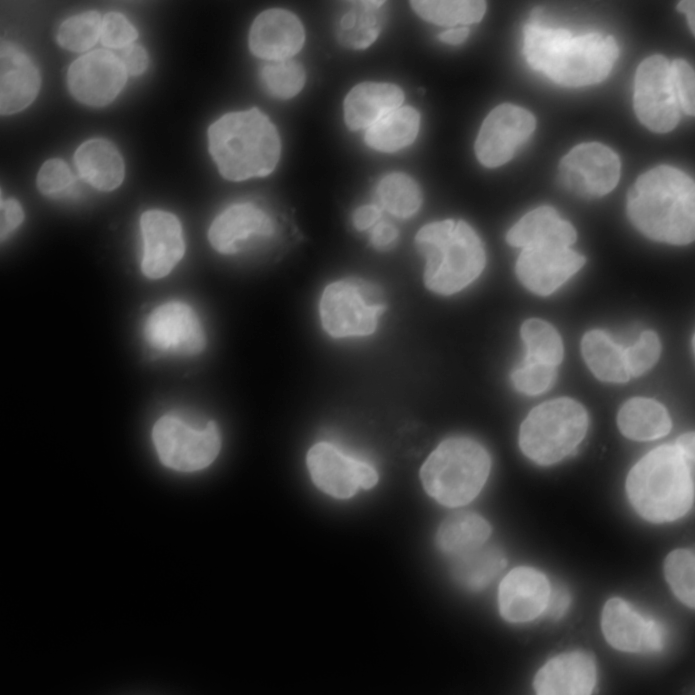
\includegraphics{bilder/segmentation/nuclei-mask/normalized.png} & 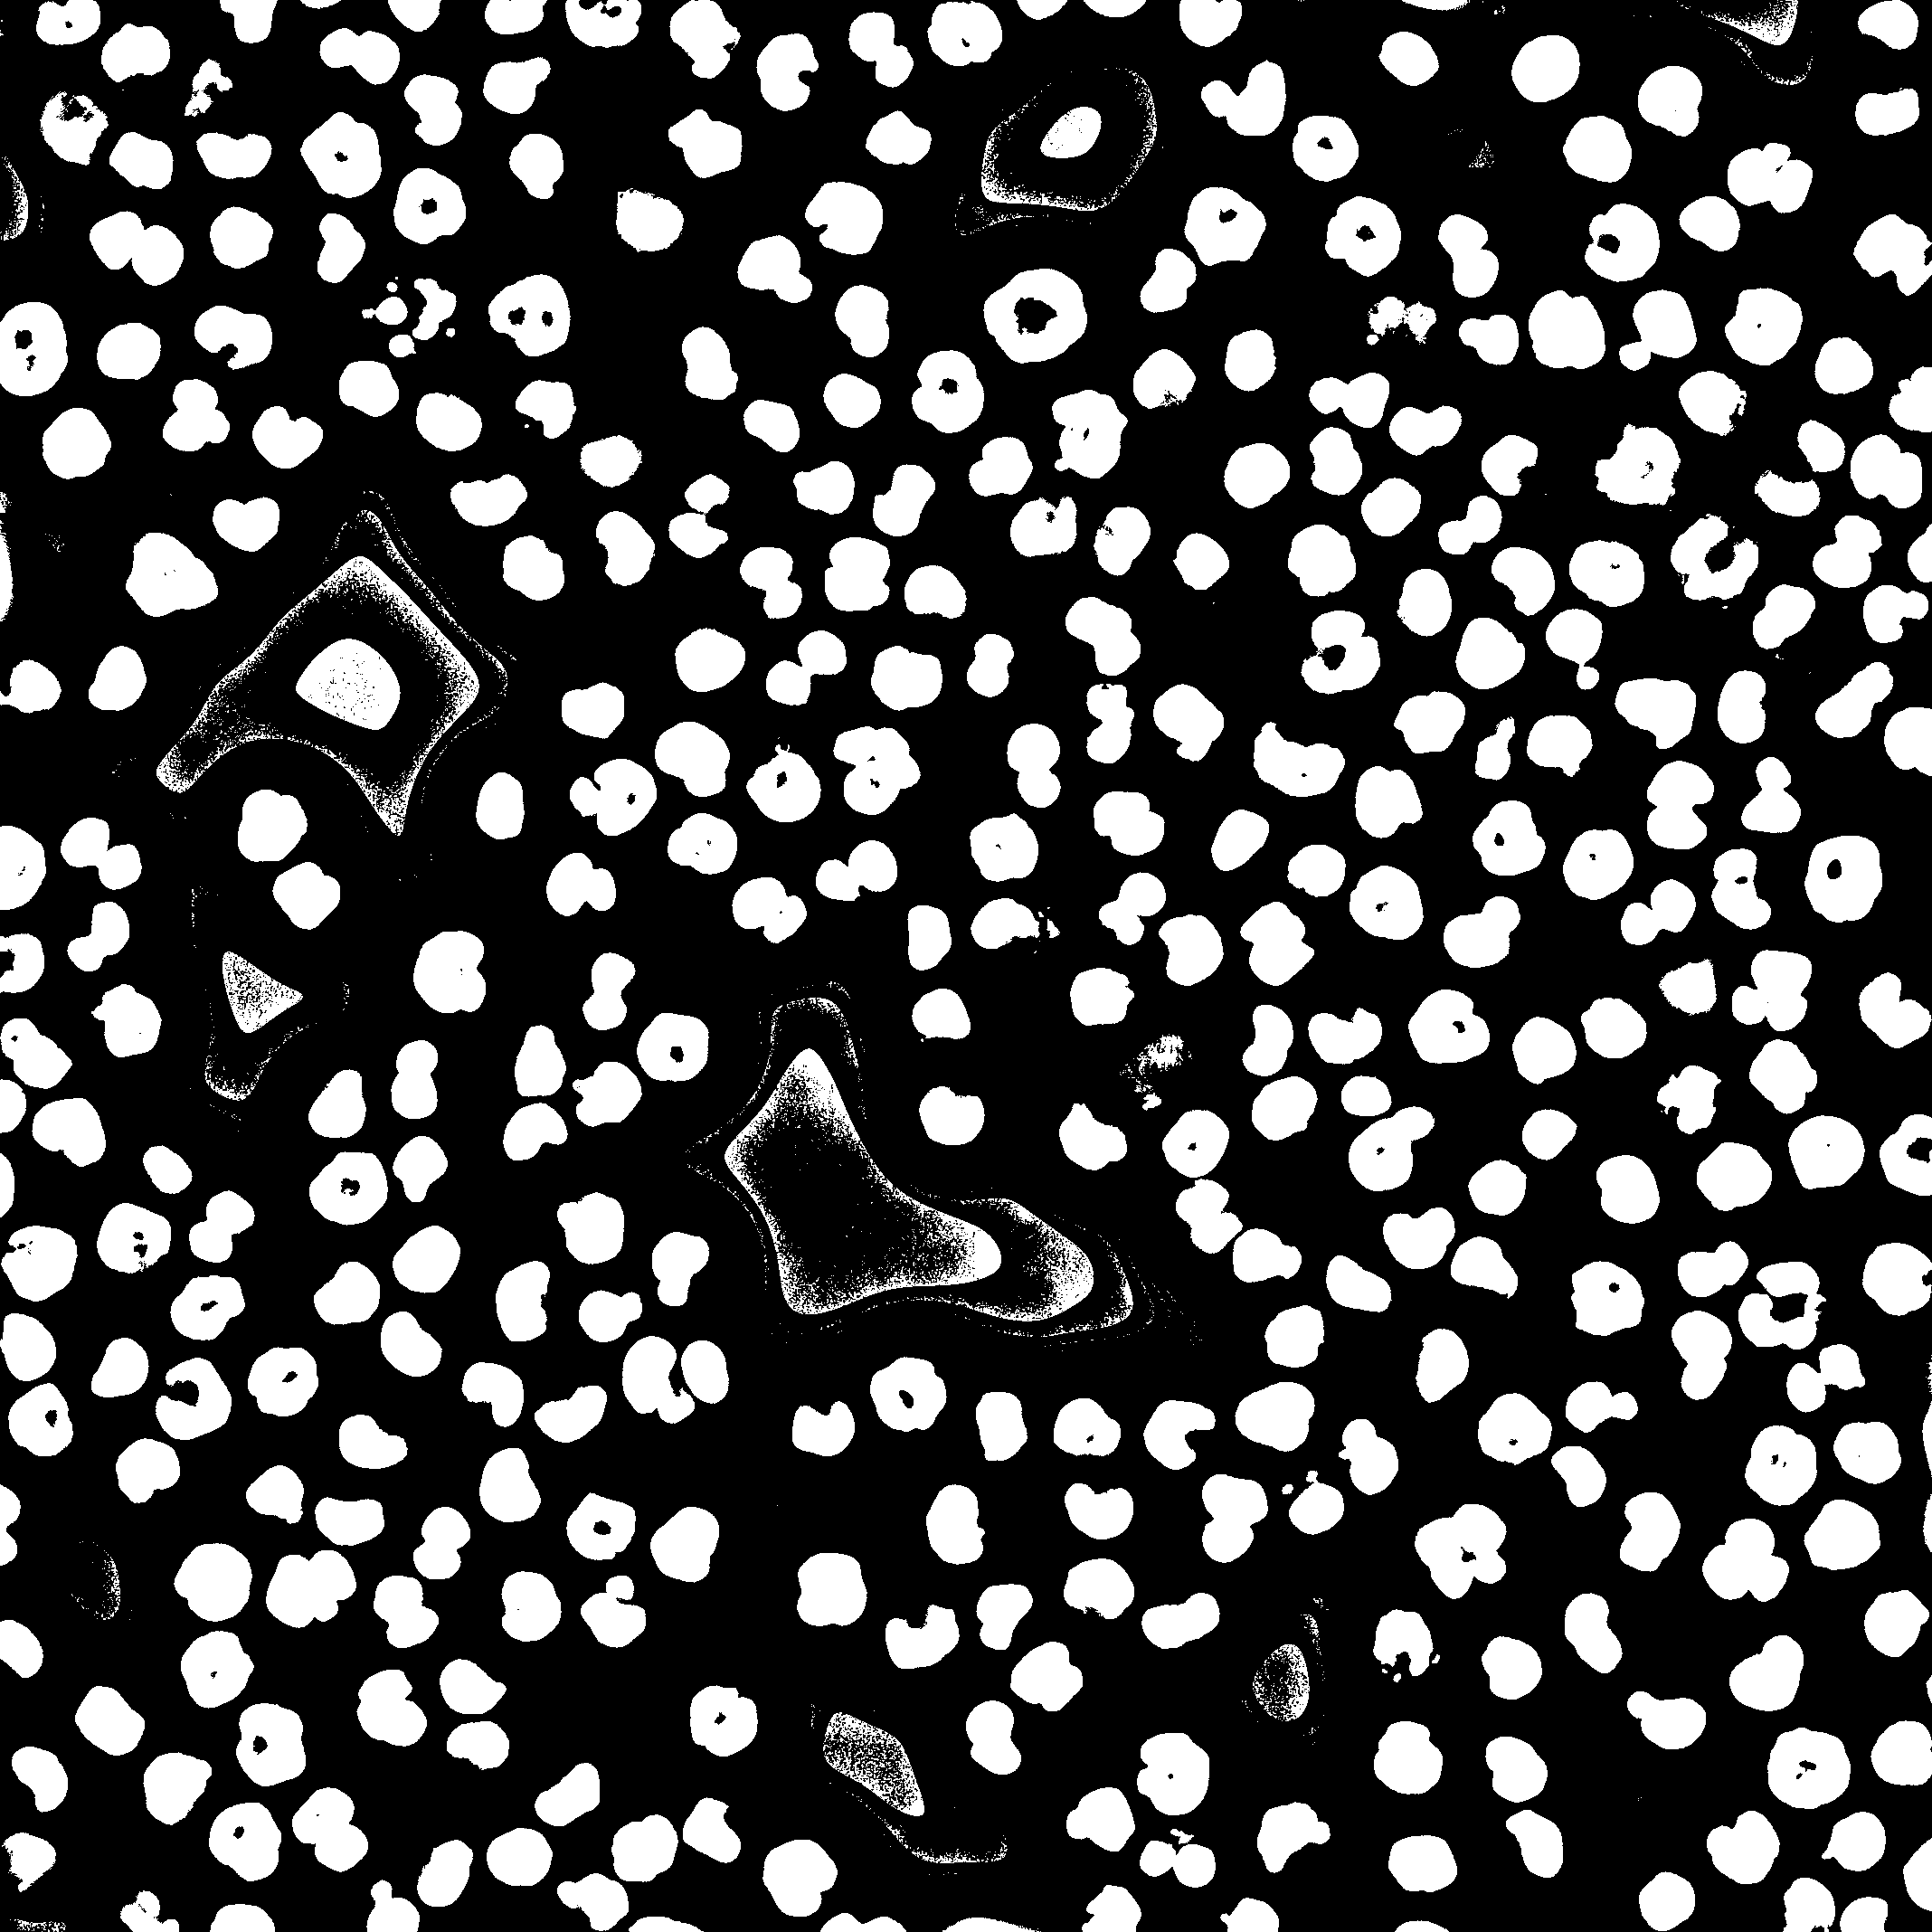
\includegraphics{bilder/segmentation/nuclei-mask/binary_local.png} &
            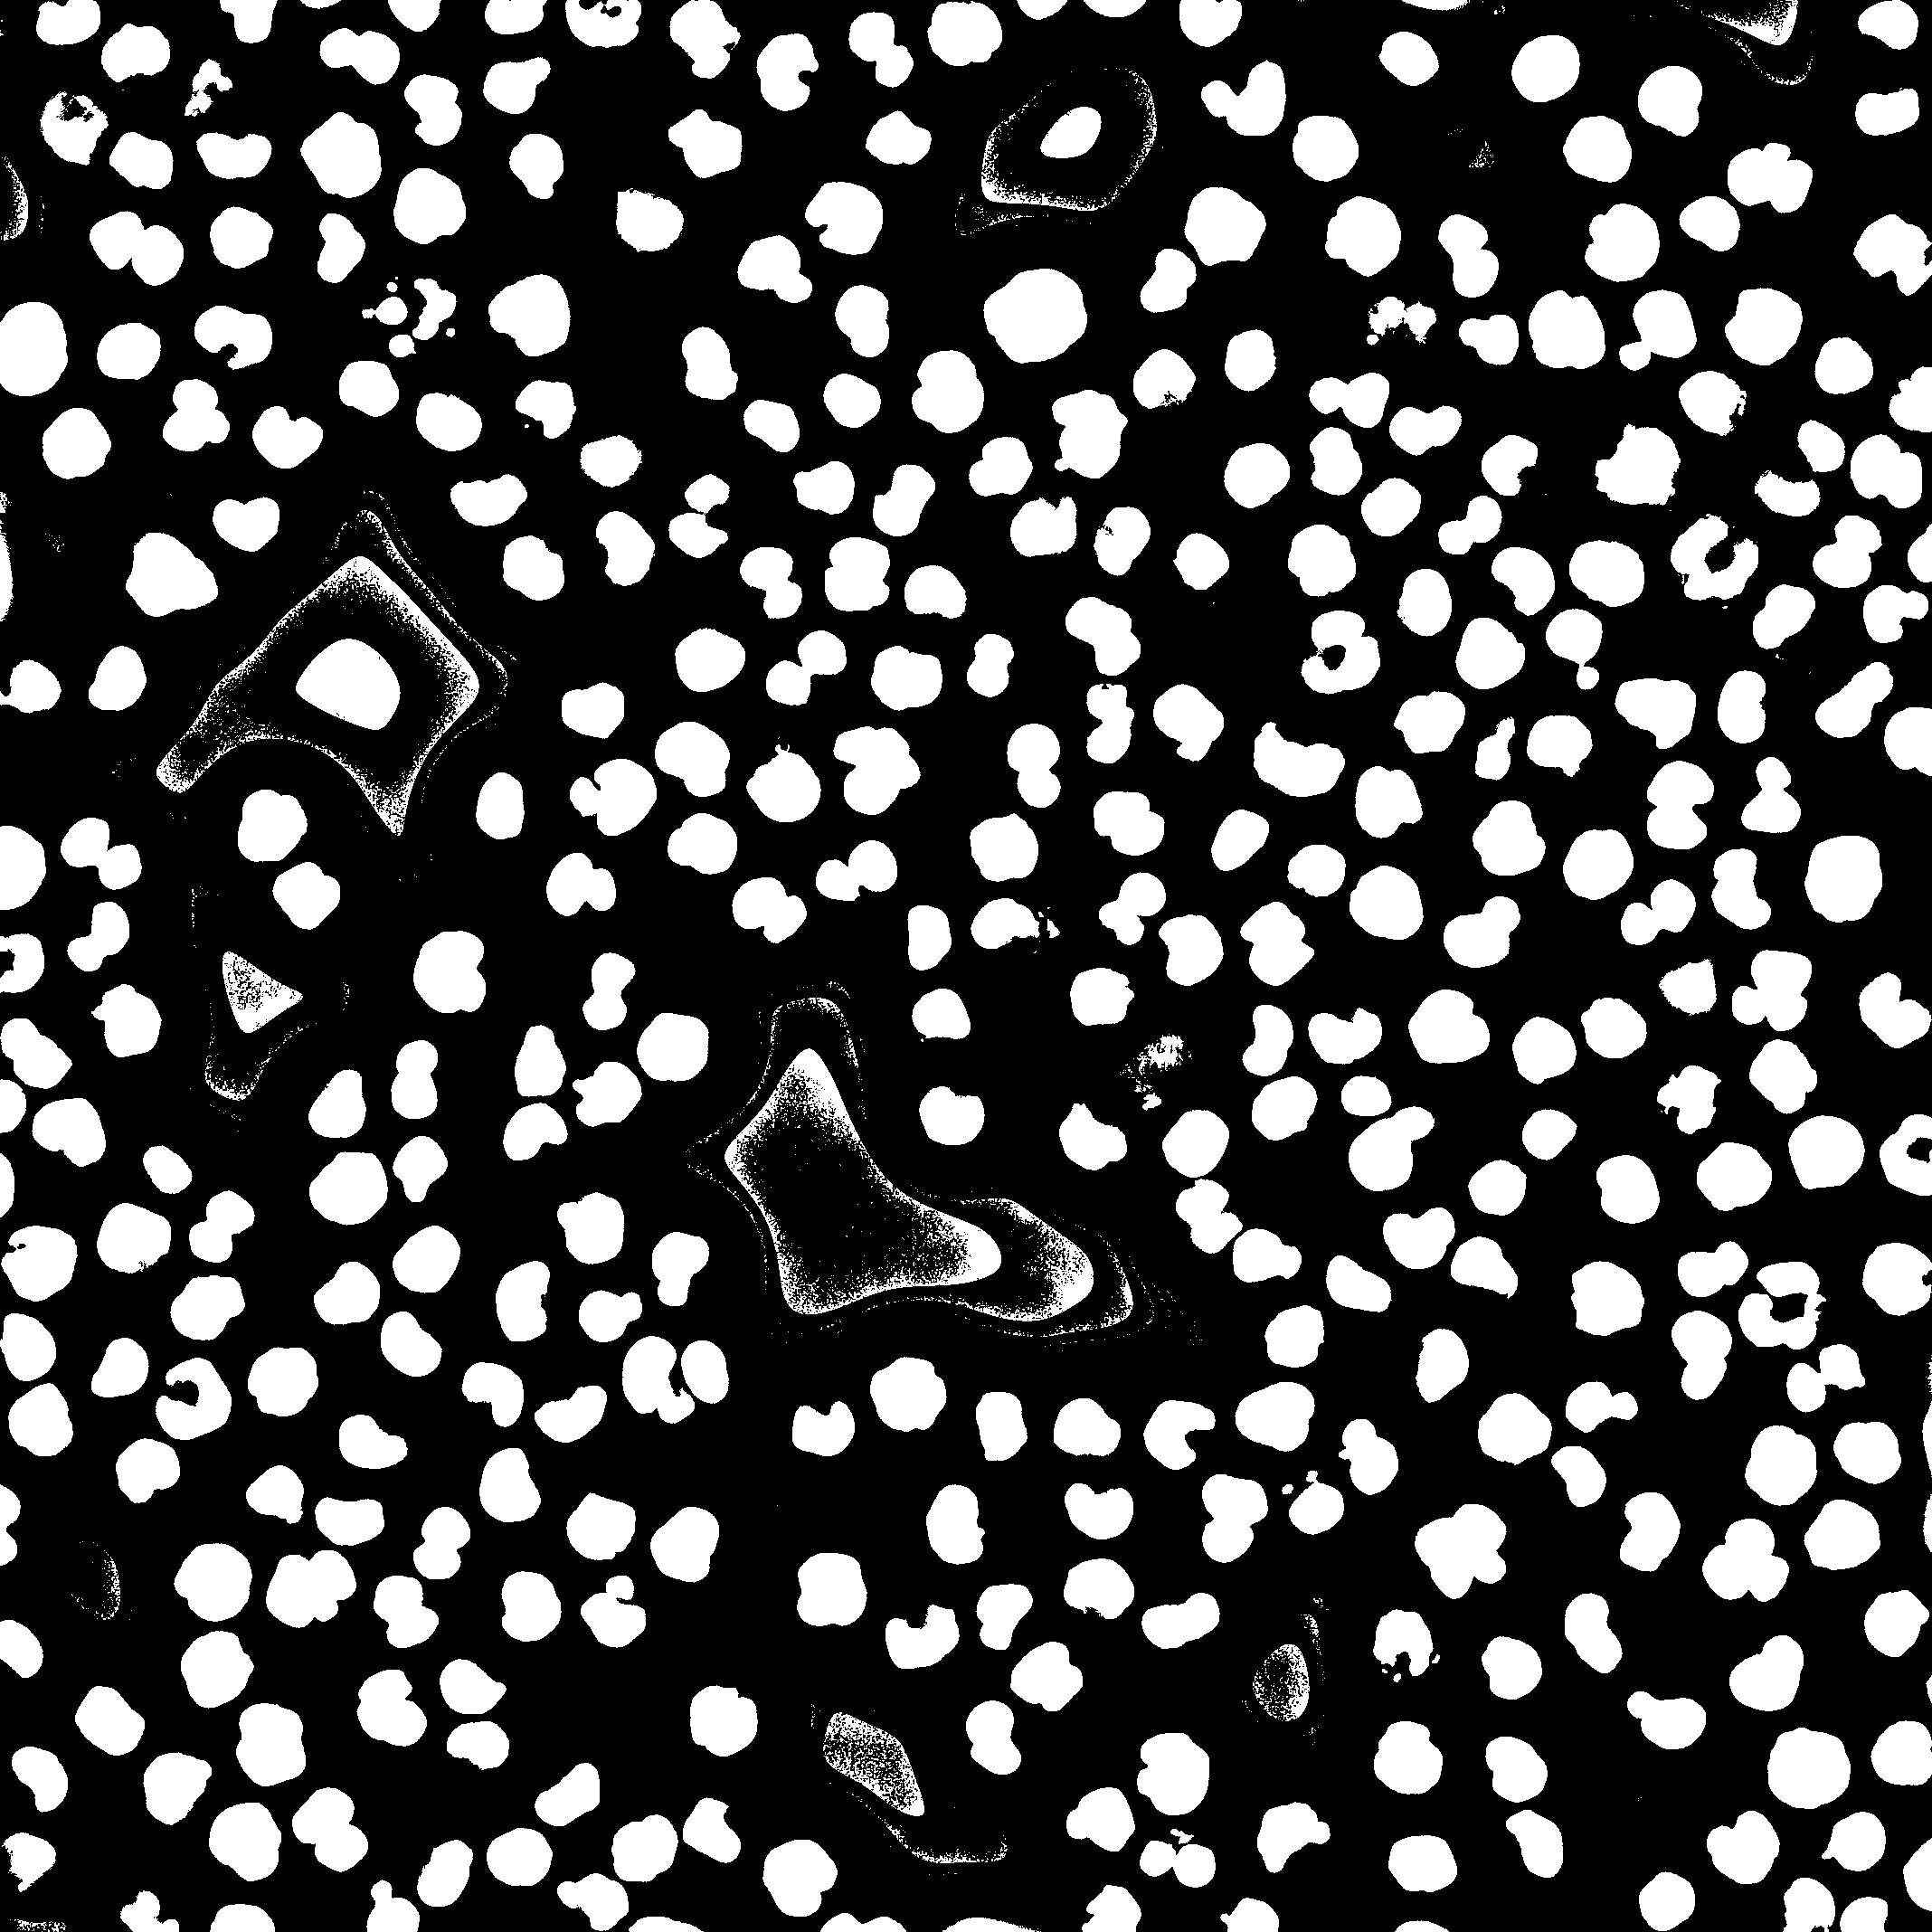
\includegraphics{bilder/segmentation/nuclei-mask/filled_holes.png} &
            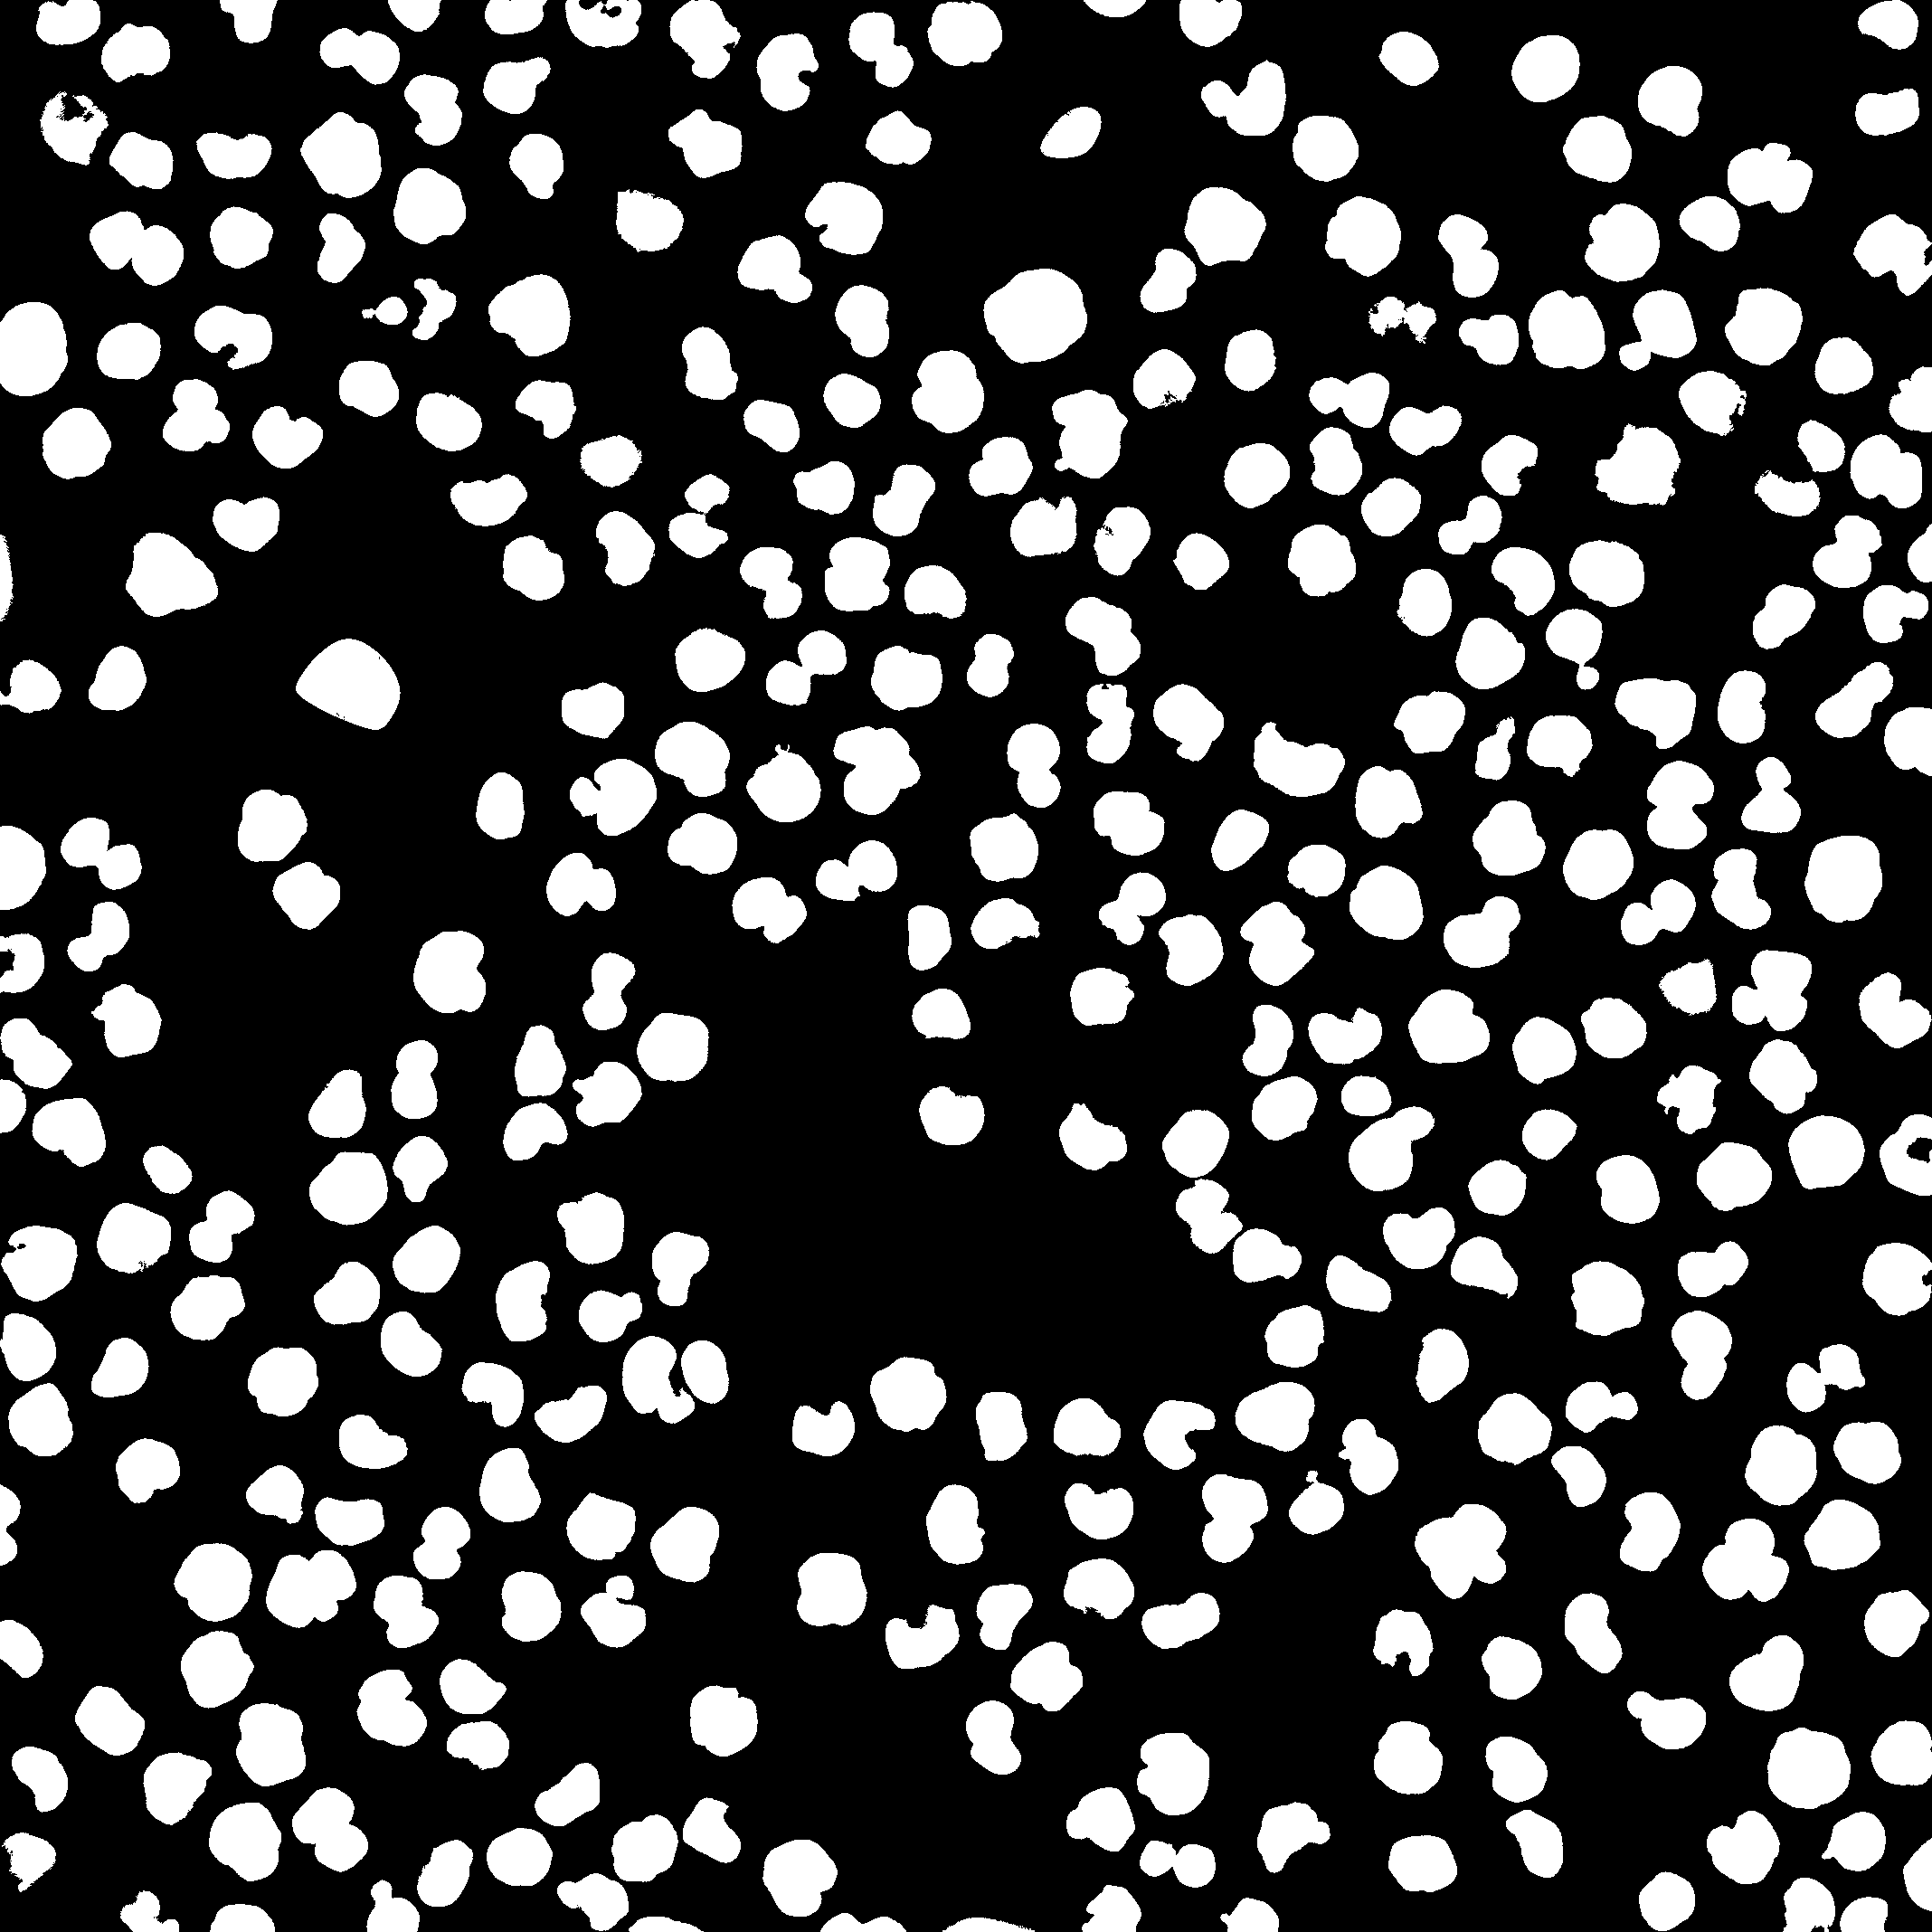
\includegraphics{bilder/segmentation/nuclei-mask/mask.png}
        \end{tabularx}
    \caption{Fluorescence segmentation}
    \label{fig:segmentation-nuclei-steps}
\end{figure}

A more detailed description of step 2 of the algorithm (thresholding) as well as the general theory behind it is provided in the next subsection.
